\documentclass[tikz]{standalone}
\usepackage{tikz}
\begin{document}
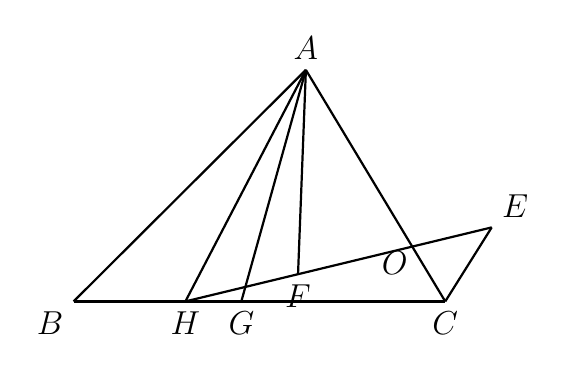
\begin{tikzpicture}[line width=0.8pt, font=\large]
  % Coordinates
  \coordinate (A) at (2.95,2.94);
  \coordinate (B) at (0,0);
  \coordinate (H) at (1.42,0);   % formerly D
  \coordinate (G) at (2.13,0);
  \coordinate (F) at (2.85,0.34);
  \coordinate (C) at (4.72,0);
  \coordinate (E) at (5.31,0.94);

  % Segments
  \draw (A) -- (B);
  \draw (A) -- (H);
  \draw (A) -- (G);
  \draw (A) -- (F);
  \draw (A) -- (C);
  \draw (B) -- (C);
  \draw (H) -- (E);
  \draw (C) -- (E);

  % Labels
  \node[above] at (A) {$A$};
  \node[below left] at (B) {$B$};
  \node[below] at (H) {$H$};
  \node[below] at (G) {$G$};
  \node[below] at (F) {$F$};
  \node[below] at (C) {$C$};
  \node[above right] at (E) {$E$};
  \node at (4.08,0.49) {$O$};
\end{tikzpicture}
\end{document}
